\chapter*{The 3 practices of BDD}


\ifnotes
    Learning outcomes:
    
    \begin{itemize}
        \item Define the three practices of BDD, and the order they should be adopted
        \item Explain how discovery and exploration are connected and collaborative 
        \item Describe how automated tests drive out implementation
        \item Show that collaborative Discovery is the pre-requisite, mandatory practice for BDD, while business-readable Gherkin and automated living documentation are valuable, downstream outputs
    \end{itemize}
    
   Setup:
   
   Print out/bring along a deck of cards that have words/phrases on each of them:
   
   The words/phrases suggested are:
   
    \begin{itemize}
        \item Discovery: Examples, Business rules, Questions, Conversation
       \item Formulation: Given/When/Then, Scenarios, Domain language, Business readable, Documentation
       \item Automation: Test-driven development, Cucumber, JUnit, Step definitions, Code
    \end{itemize}
   
   Give a deck each to each group. Ask them to sort them into 4 piles - one for each of the BDD practices, and one for "not sure".
   
   See \emph{Card Sort - Jigsaw} in TFTBOTR
\fi

\ifcontent
    The BDD approach is made up of three practices, shown in the diagram below. Only the first, \emph{Discovery}, is mandatory. The subsequent practices deliver incremental value and facilitate continuous delivery and continuous deployment.
    
    \begin{center}
        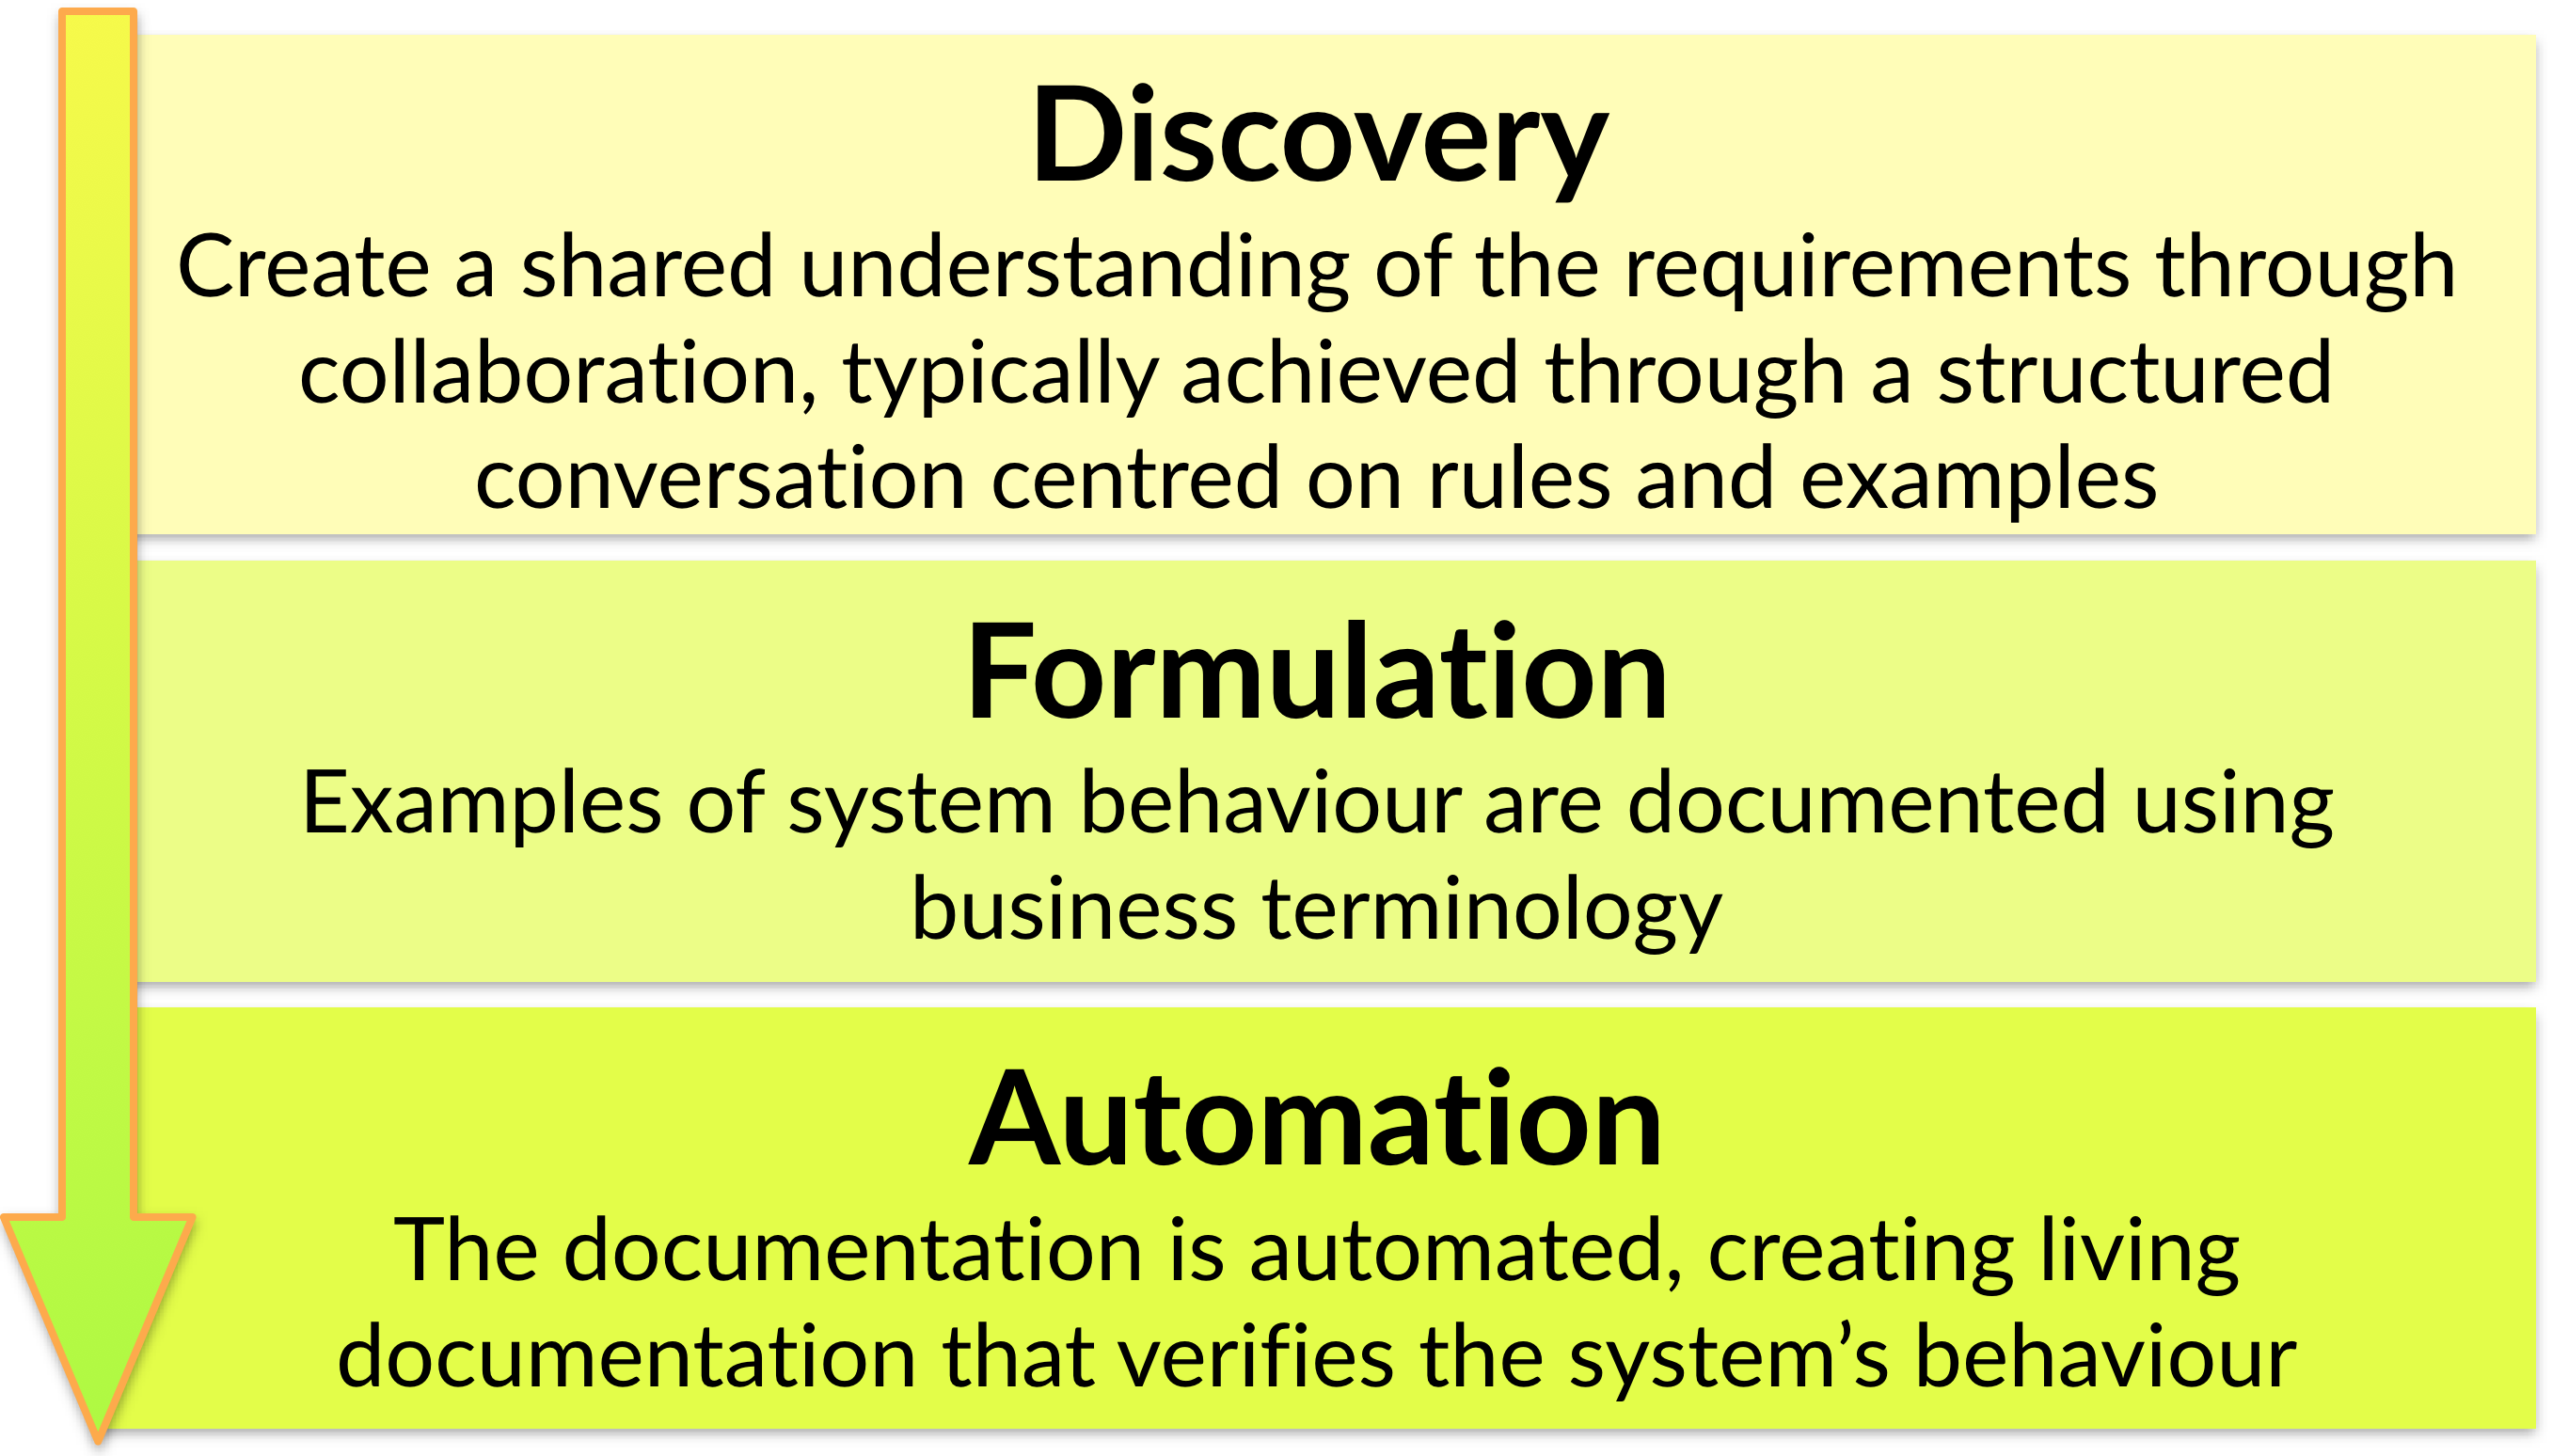
\includegraphics[width=\textwidth, keepaspectratio]{images/three-practices}
    \end{center}
    
    \QandAbox{How could \emph{Discovery} be valuable in the absence of \emph{Formulation} and \emph{Automation}?}{1.7}
    
    \QandAbox{What substantial extra value can \emph{Formulation} and \emph{Automation} bring?}{1.7}
    
    \QandAbox{When might it not be appropriate to pursue \emph{Formulation} and \emph{Automation}?}{1.7}
\fi 
